\documentclass[10pt,aspectratio=169]{beamer}
% Packages
\usepackage{mathabx}
\usepackage{xcolor}
\usepackage{amsmath}
\usepackage{mathtools}
\usepackage{standalone}
\usepackage{mhchem}
\usepackage{textpos}
\usepackage{graphicx}
\usepackage{wrapfig}
\graphicspath{{images}}

% Configure template
\setbeamertemplate{navigation symbols}{}

% Theme
\usetheme[progressbar=frametitle]{metropolis}
\setbeamertemplate{caption}[numbered]
\setbeamersize{text margin left=5mm,text margin right=5mm}

% Title page details: 
\title{Scientific Computing: Molecular dynamics}
\subtitle{Problemsheet 2}
\author{Jimin Kim, Christian Nix, Noah Schlenker}
\date{17. Mai 2024}
\institute{Technical University of Munich}

\begin{document}

% Title page frame
\maketitle

\addtobeamertemplate{frametitle}{}{
\begin{textblock*}{100mm} (.945\textwidth,-.85cm)

\includegraphics[scale=0.14]{../template/res/tum_logo.png}
\end{textblock*}}

% Outline frame
\begin{frame}{Outline}
    \tableofcontents
\end{frame}

%Slides for Unit tests
\section{Unit Tests}

\begin{frame}
    \frametitle{Google test for general testing}

        Integration of \emph{gtest} via CMake after checking presence in system

    \begin{figure}[H]
        
\includegraphics[width=\textwidth]{res/gtest3.png}
    \end{figure}


\end{frame}

\begin{frame}
    \frametitle{Google test for general testing}

        Handling src files as a library so that tests can be executed separately

    \begin{figure}[H]
        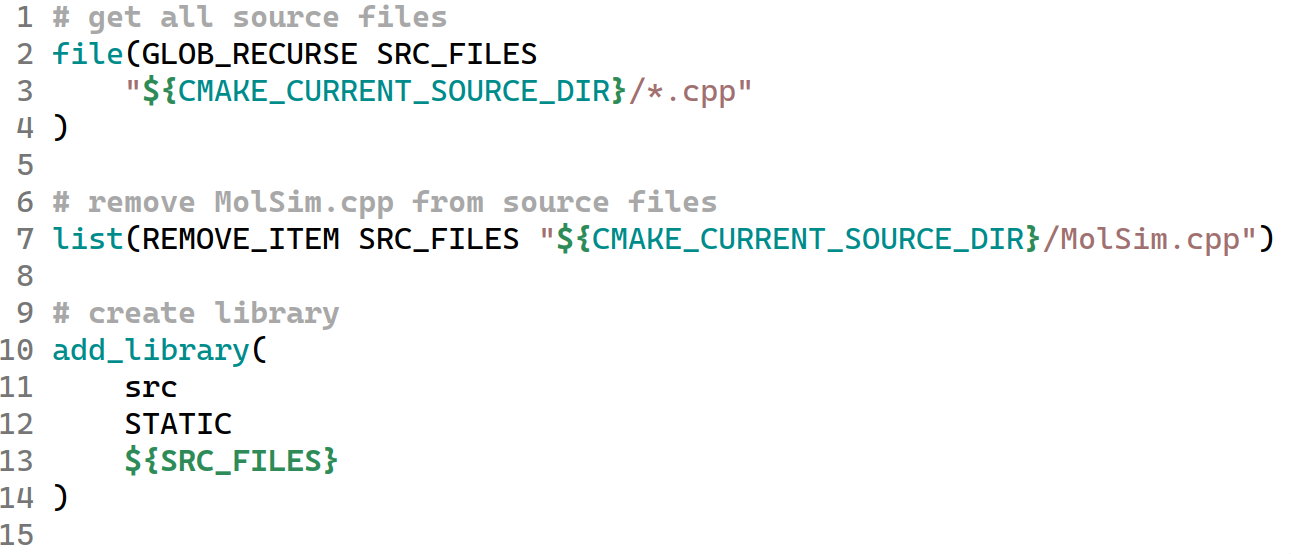
\includegraphics[width=\textwidth]{res/gtest1.png}
    \end{figure}


\end{frame}

\begin{frame}
    \frametitle{Google test for general testing}

        Handling src files as a library so that tests can be executed separately

    Linking with MolSim:
    \begin{figure}[H]
        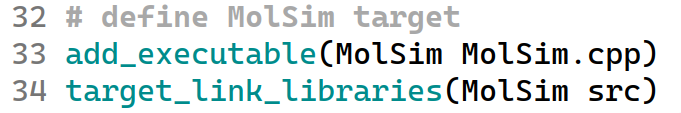
\includegraphics[width=0.5\textwidth]{res/gtest2.png}
    \end{figure}

    Linking with tests:
    \begin{figure}[H]
        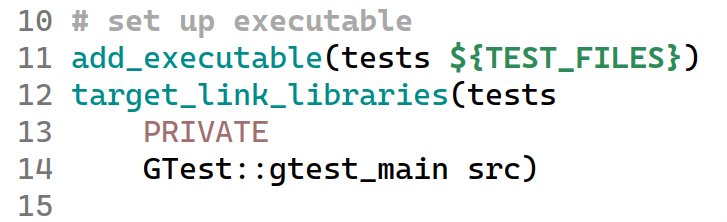
\includegraphics[width=0.5\textwidth]{res/gtest4.png}
    \end{figure}

\end{frame}



%Slides for CI
\section{Continuous Integration}

\begin{frame}
    \frametitle{Docker and act}

    \begin{itemize}
        \item Not much to mention: CI realization through Docker and 'nektos/act'
        \item Branch protection rules on \emph{master} and \emph{assignment*} branches
    \end{itemize}

\end{frame}

%Slides for spdlog
\section{Spdlog}

\begin{frame}
    \frametitle{spdlog functions vs macros}

    \begin{itemize}
        \item Incorporation using CMake module, including pre-fetch check for availability
        \item Macro benefits: Compile-time and run-time benefits
        \item Function benefits: type safety
        \item Run-time adjustment of log levels $\Rightarrow$ Compile-time benefits of macros not relevant
        \item Current project status undergoes frequent changes $\Rightarrow $safety preferred
    \end{itemize}
    \bigskip

    $\Rightarrow$ Log-level can be specified by user with option \texttt{-l}

\end{frame}



% Slides for References
\section{References}	
	\begin{thebibliography}
		\frame{
			\bibitem{StraPattern} https://refactoring.guru/design-patterns/strategy
		}
	\end{thebibliography}

\end{document}